%(BEGIN_QUESTION)
% Copyright 2015, Tony R. Kuphaldt, released under the Creative Commons Attribution License (v 1.0)
% This means you may do almost anything with this work of mine, so long as you give me proper credit

\textit{R-verdi} for et isolasjonsmateriale er definert som forholdet mellom lengde ($l$) og varmeledningsevne ($k$), begge hentet fra varmeledning-likningen:

$$R = {l \over k}$$

$${dQ \over dt} = {kA {\Delta T} \over l}$$

Omskriv varmeledning-likningen slik at den bruker $R$ i stedet for $k$, og bruk den deretter til å beregne varmetapet gjennom flatene i boksen under, som er isolert med R-30-isolasjon ($R$ = 30 ft$^{2}$ $\cdot$ h $\cdot$ F$^{o}$ / Btu), oppvarmet innvendig til 75$^{o}$ F og utsatt for utetemperatur (omgivelse) på 40$^{o}$ F:

$$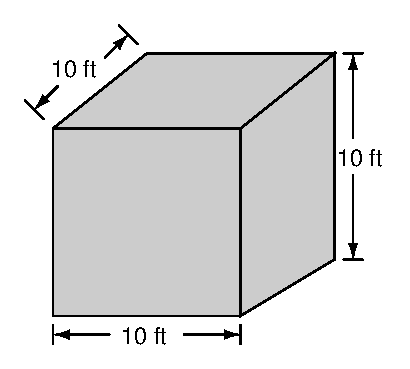
\includegraphics[width=15.5cm]{i00333x01.eps}$$

Ekstraoppgave: Hvis boksen varmes kun av en elektrisk lyspære, hvor stor må lyspæren være (altså effekt i watt) for å holde boksens innvendige temperatur på 75$^{o}$ F ved utetemperatur 40$^{o}$ F?

\vskip 20pt \vbox{\hrule \hbox{\strut \vrule{} {\bf Forslag til sokratisk diskusjon} \vrule} \hrule}

\begin{itemize}
\item{} Beskriv sammenhengen mellom isolasjonens R-verdi og energieffektivitet for et oppvarmet bygg.
\item{} Beskriv sammenhengen mellom isolasjonens R-verdi og energieffektivitet for et avkjølt (airconditionert) bygg.
\item{} Anta at boksen varmes av et elektrisk varmeelement med av/på-termostat som holder lufttemperaturen ved eller nær 75 grader F. Hvordan vil \textit{arbeidssyklusen} til varmeren (på-tid delt på summen av på+av-tid) variere når utetemperaturen endres?
\item{} Vis hvordan man kan \textit{anslå} tallsvaret i denne oppgaven uten kalkulator.
\end{itemize}

\underbar{file i00333}
%(END_QUESTION)





%(BEGIN_ANSWER)

Svar på ekstraoppgaven: Lyspæren måtte vært på 205 watt (to 100-watts pærer samtidig ville kommet nær).

%(END_ANSWER)





%(BEGIN_NOTES)

En enkel måte å erstatte $k$ og $l$ med $R$ er å løse for $l$ uttrykt ved $R$ og $k$ ($l = kR$), deretter sette $kR$ inn i ledningslikningen i stedet for $l$, og stryke $k$ i teller og nevner:

$${dQ \over dt} = {A {\Delta T} \over R}$$

Boksens totale areal ($A$) er 600 kvadratfot (seks sider, hver med overflateareal på 100 kvadratfot). Temperaturdifferansen over boksveggene er 35 grader (75 $-$ 40). R-verdien er gitt som R-30:

$${dQ \over dt} = {(600) (35) \over 30} = 700 \hbox{ BTU/hour}$$

Omregningsfaktor mellom BTU/h og watt er 745.7 watt = 2544.43 BTU/h. Dermed:

$$\left({700 \hbox{ BTU/h} \over 1}\right) \left( {745.7 \hbox{ W} \over 2544.43 \hbox{ BTU/h}} \right) = 205.15 \hbox{ W}$$






\vfil \eject

\noindent
{\bf Oppsummeringsquiz:}

Anta at et hus trenger 12,500 BTU per time i varmetilførsel for å holde romtemperaturen på 70 grader Fahrenheit når utetemperaturen er 30 grader Fahrenheit. Beregn omtrent hvor stor varmetilførsel som kreves for å holde samme romtemperatur dersom været blir varmere til 50 grader Fahrenheit, alt annet likt.

\begin{itemize}
\item{} 3,125 BTU per time
\vskip 5pt 
\item{} 25,000 BTU per time 
\vskip 5pt 
\item{} 6,250 BTU per time
\vskip 5pt 
\item{} 100,000 BTU per time
\vskip 5pt 
\item{} 12,500 BTU per time 
\vskip 5pt 
\item{} 50,000 BTU per time
\end{itemize}

%INDEX% Measurement, heat: conduction through a solid substance

%(END_NOTES)
